\documentclass[8pt,aspectratio=169]{beamer}
\usetheme{Madrid}
\usecolortheme{seahorse}
\setbeamertemplate{navigation symbols}{}

% Packages
\usepackage{graphicx}
\usepackage{amsmath}
\usepackage{tcolorbox}
\usepackage{tikz}
\usetikzlibrary{positioning,arrows.meta}

% Custom colors matching our Python visualizations
\definecolor{mlblue}{RGB}{68,114,196}
\definecolor{mlgreen}{RGB}{68,160,68}
\definecolor{mlorange}{RGB}{255,127,14}
\definecolor{mlred}{RGB}{214,39,40}
\definecolor{mlpurple}{RGB}{139,90,155}

% Title
\title{Transformers: Understanding Parallel Intelligence}
\subtitle{From Zero to ChatGPT - A BSc Journey}
\author{Week 5: Transformers}
\date{}

\begin{document}

% Slide 1: Title
\begin{frame}
\titlepage
\end{frame}

% ===========================================
% PART 1: THE CHALLENGE (5 slides)
% ===========================================

% Slide 2: The Google Search Experience
\begin{frame}{How Google Reads Your Mind}
\begin{columns}[T]
\column{0.48\textwidth}
\textbf{Try this:} Type in Google: ``How do transformers...''

\vspace{3mm}
\textbf{Google instantly suggests:}
\begin{itemize}
\item ``...work in machine learning''
\item ``...process language''
\item ``...learn from data''
\end{itemize}

\vspace{3mm}
\textbf{The Mystery:}
\begin{itemize}
\item Google reads ALL your words at once
\item Not word-by-word like old systems
\item Understands context instantly
\end{itemize}

\column{0.48\textwidth}
\begin{center}
\begin{tcolorbox}[colback=white,colframe=gray!75!black,width=0.9\columnwidth]
\texttt{How do transformers}\\[2mm]
\hrule\vspace{2mm}
{\small\color{gray}
\texttt{...work in machine learning}\\
\texttt{...process language}\\
\texttt{...learn from data}\\
\texttt{...handle attention}\\
}
\end{tcolorbox}
\end{center}

\vspace{3mm}
\begin{tcolorbox}[colback=yellow!10!white,colframe=orange!75!black]
\textbf{Question:} How does it understand whole sentences simultaneously?
\end{tcolorbox}
\end{columns}
\end{frame}

% Slide 3: Words as Coordinates in Space
\begin{frame}{Discovery 1: Words Live in Space}
\begin{columns}[T]
\column{0.48\textwidth}
\textbf{Think about GPS coordinates:}
\begin{itemize}
\item Paris: (48.8°N, 2.3°E, 35m altitude)
\item London: (51.5°N, 0.1°W, 11m altitude)
\item Similar cities are nearby in space
\end{itemize}

\vspace{3mm}
\textbf{Words work the same way!}
\begin{itemize}
\item ``cat'': [0.7, 0.2, 0.5] in meaning space
\item ``dog'': [0.8, 0.3, 0.4] (nearby - similar!)
\item ``car'': [0.1, 0.9, 0.2] (far - different!)
\end{itemize}

\vspace{3mm}
\textbf{This is called:} \colorbox{mlblue!20}{Word Embeddings}

\column{0.48\textwidth}
\begin{center}
\includegraphics[width=0.95\columnwidth]{../figures/3d_word_space.pdf}
\end{center}
\end{columns}
\end{frame}

% Slide 4: Relationships Between All Words
\begin{frame}{Discovery 2: Every Word Connects to Every Other}
\begin{center}
\includegraphics[width=0.85\textwidth]{../figures/3d_connection_network.pdf}
\end{center}

\vspace{3mm}
\begin{columns}[T]
\column{0.48\textwidth}
\textbf{In ``The cat sat on the mat'':}
\begin{itemize}
\item 6 words = 15 connections!
\item Each word must consider all others
\item Some connections strong, some weak
\end{itemize}

\column{0.48\textwidth}
\textbf{The Explosion:}
\begin{itemize}
\item 10 words = 45 connections
\item 100 words = 4,950 connections
\item 1000 words = 499,500 connections!
\end{itemize}
\end{columns}
\end{frame}

% Slide 5: Information Overload Problem
\begin{frame}{The Problem: Information Overload}
\begin{center}
\includegraphics[width=0.85\textwidth]{../figures/exponential_explosion_3d.pdf}
\end{center}

\vspace{2mm}
\begin{columns}[T]
\column{0.48\textwidth}
\textbf{Computational Explosion:}
\begin{itemize}
\item 10 words = 45 connections
\item 100 words = 4,950 connections
\item 1000 words = 499,500 connections!
\item Formula: n(n-1)/2
\end{itemize}

\column{0.48\textwidth}
\begin{tcolorbox}[colback=red!10!white,colframe=red!75!black]
\textbf{Crisis:} Processing everything is impossible at scale!
\end{tcolorbox}

\vspace{3mm}
\textbf{Forward Question:} Can we be selective instead of exhaustive?
\end{columns}
\end{frame}

% ===========================================
% PART 2: FIRST ATTEMPT (4 slides)
% ===========================================

% Slide 6: The Naive Approach
\begin{frame}{First Attempt: Connect Everything}
\begin{center}
\includegraphics[width=0.95\textwidth]{../figures/chaos_network_3d.pdf}
\end{center}

\vspace{2mm}
\textbf{The Naive Idea:} Connect every word to every other - surely more connections = better understanding?

\vspace{2mm}
\begin{columns}[T]
\column{0.48\textwidth}
\textbf{5 Words:} Clear patterns, manageable
\column{0.48\textwidth}
\textbf{20 Words:} Complete chaos, signal lost in noise
\end{columns}
\end{frame}

% Slide 7: Computing All Relationships
\begin{frame}{Computing All Relationships}
\begin{columns}[T]
\column{0.48\textwidth}
\textbf{For ``The cat sat'':}
\begin{center}
\begin{tabular}{|l|c|c|c|}
\hline
 & The & cat & sat \\
\hline
The & 1.0 & 0.3 & 0.2 \\
cat & 0.3 & 1.0 & 0.7 \\
sat & 0.2 & 0.7 & 1.0 \\
\hline
\end{tabular}
\end{center}

\vspace{3mm}
\textbf{Each number = relationship strength}
\begin{itemize}
\item ``cat'' - ``sat'' = 0.7 (strong!)
\item ``The'' - ``sat'' = 0.2 (weak)
\end{itemize}

\column{0.48\textwidth}
\textbf{Matrix grows quadratically:}
\begin{itemize}
\item 3 words = 3×3 matrix
\item 100 words = 100×100 matrix
\item 1000 words = 1,000,000 numbers!
\end{itemize}

\vspace{3mm}
\begin{tcolorbox}[colback=yellow!10!white]
Complete matrix for every sentence!
\end{tcolorbox}
\end{columns}
\end{frame}

% Slide 8: SUCCESS on Short Sequences
\begin{frame}{SUCCESS! (On Simple Cases)}
\begin{columns}[T]
\column{0.48\textwidth}
\textbf{Works Great For:}
\begin{itemize}
\item ``The cat'' $\rightarrow$ predicts ``sat'' \checkmark (95\%)
\item ``Water is'' $\rightarrow$ predicts ``wet'' \checkmark (92\%)
\item ``Birds can'' $\rightarrow$ predicts ``fly'' \checkmark (89\%)
\item ``Coffee tastes'' $\rightarrow$ predicts ``good'' \checkmark (91\%)
\end{itemize}

\vspace{3mm}
\textbf{Why it works:}
\begin{itemize}
\item Few connections to track
\item Clear patterns visible
\item No information overload yet
\end{itemize}

\column{0.48\textwidth}
\begin{center}
\colorbox{green!20}{\parbox{0.9\columnwidth}{
\textbf{Celebration!} \\
\vspace{2mm}
We can predict words! \\
The approach seems valid! \\
Let's scale it up!
}}
\end{center}
\end{columns}
\end{frame}

% Slide 9: FAILURE - The Noise Problem
\begin{frame}{FAILURE: Signal Lost in Noise}
\begin{columns}[T]
\column{0.48\textwidth}
\textbf{Performance Collapse:}
\begin{center}
\begin{tabular}{|l|r|r|r|}
\hline
\textbf{Length} & \textbf{Signal} & \textbf{Noise} & \textbf{Accuracy} \\
\hline
10 words & 3 & 7 & 85\% \\
50 words & 5 & 45 & 42\% \\
100 words & 8 & 92 & 18\% \\
500 words & 15 & 485 & 3\% \\
\hline
\end{tabular}
\end{center}

\vspace{3mm}
\textbf{The Pattern:} More words = More noise!

\column{0.48\textwidth}
\textbf{What Goes Wrong:}
\begin{itemize}
\item Important connections drowned out
\item 95\% of connections irrelevant
\item Can't find what matters
\item Like finding needle in haystack
\end{itemize}

\vspace{3mm}
\begin{tcolorbox}[colback=red!10!white,colframe=red!75!black]
\textbf{Diagnosis:} We need to be SELECTIVE, not exhaustive!
\end{tcolorbox}
\end{columns}
\end{frame}

% ===========================================
% PART 3: THE BREAKTHROUGH (11 slides)
% ===========================================

% Slide 10: Human Reading Experiment
\begin{frame}{How Do Humans Actually Read?}
\begin{center}
\includegraphics[width=0.95\textwidth]{../figures/attention_heatmap.pdf}
\end{center}

\vspace{2mm}
\begin{columns}[T]
\column{0.48\textwidth}
\textbf{Key Realization:}
\begin{itemize}
\item Humans SELECTIVELY FOCUS!
\item We spotlight what matters
\item Ignore decorative adjectives
\item Focus on functional words
\end{itemize}

\column{0.48\textwidth}
\begin{tcolorbox}[colback=yellow!10!white,colframe=orange!75!black]
\textbf{The Insight:} What if computers could learn WHERE to look like humans do?
\end{tcolorbox}
\end{columns}
\end{frame}

% Slide 11: The Attention Hypothesis
\begin{frame}{The Hypothesis: Selective Attention}
\begin{center}
\includegraphics[width=0.8\textwidth]{../figures/3d_attention_spotlight.pdf}
\end{center}

\vspace{3mm}
\begin{columns}[T]
\column{0.48\textwidth}
\textbf{Old Way (Everything):}
\begin{itemize}
\item Process all connections
\item Equal weight to all
\item Information overload
\end{itemize}

\column{0.48\textwidth}
\textbf{New Way (Selective):}
\begin{itemize}
\item Adjustable spotlights
\item Focus on what matters
\item Ignore the irrelevant
\end{itemize}
\end{columns}
\end{frame}

% Slide 12: Attention as Percentages
\begin{frame}{Breaking It Down: Attention as Percentages}
\begin{center}
\includegraphics[width=0.85\textwidth]{../figures/attention_pie_3d.pdf}
\end{center}

\vspace{2mm}
\begin{columns}[T]
\column{0.48\textwidth}
\textbf{For predicting ``mat'':}
\begin{itemize}
\item ``on'': 35\% attention
\item ``the'': 25\% attention
\item ``sat'': 20\% attention
\item ``cat'': 15\% attention
\item ``The'': 5\% attention
\end{itemize}

\column{0.48\textwidth}
\begin{tcolorbox}[colback=mlblue!10!white]
\textbf{Key Properties:}
\begin{itemize}
\item Percentages sum to 100\%
\item Higher \% = more important
\item Learned from data
\end{itemize}
\end{tcolorbox}
\end{columns}
\end{frame}

% Slide 13: How to Calculate Relevance
\begin{frame}{The Math: How Similar Are Two Words?}
\begin{center}
\includegraphics[width=0.9\textwidth]{../figures/vector_angles_3d.pdf}
\end{center}

\vspace{2mm}
\begin{columns}[T]
\column{0.48\textwidth}
\textbf{Dot Product = Similarity:}
\begin{itemize}
\item Small angle = High similarity
\item Large angle = Low similarity
\item Formula: Q · K = |Q| × |K| × cos($\theta$)
\end{itemize}

\column{0.48\textwidth}
\textbf{Key Insight:}
\begin{itemize}
\item Similar direction = Strong attention
\item Opposite direction = Weak attention
\item Works in 512 dimensions too!
\end{itemize}
\end{columns}
\end{frame}

% Slide 14: Query-Key-Value Mechanism
\begin{frame}{The Three Questions: Query, Key, Value}
\begin{center}
\includegraphics[width=0.9\textwidth]{../figures/qkv_transformation_3d.pdf}
\end{center}

\vspace{2mm}
\begin{columns}[T]
\column{0.33\textwidth}
\textbf{Query (Q):}
``What am I looking for?''
\begin{itemize}
\item Seeks information
\item Defines needs
\end{itemize}

\column{0.33\textwidth}
\textbf{Key (K):}
``What do I contain?''
\begin{itemize}
\item Advertises content
\item Signals relevance
\end{itemize}

\column{0.33\textwidth}
\textbf{Value (V):}
``What info do I provide?''
\begin{itemize}
\item Actual information
\item Content to aggregate
\end{itemize}
\end{columns}

\vspace{2mm}
\begin{center}
\colorbox{yellow!10}{\parbox{0.7\textwidth}{\centering Q·K determines attention weights, V provides the actual information}}
\end{center}
\end{frame}

% Slide 15: Computing Attention Scores
\begin{frame}{Step-by-Step: Computing Attention}
\begin{center}
\includegraphics[width=0.95\textwidth]{../figures/attention_flow_diagram.pdf}
\end{center}

\vspace{2mm}
\begin{columns}[T]
\column{0.48\textwidth}
\textbf{The Process:}
\begin{enumerate}
\item Q meets all K's (dot product)
\item Calculate relevance scores
\item Apply softmax (to percentages)
\item Weight the values
\item Sum to get output
\end{enumerate}

\column{0.48\textwidth}
\begin{tcolorbox}[colback=green!10!white]
\textbf{Result:} Context-aware representation that knows ``mat'' likely follows ``on the''!
\end{tcolorbox}
\end{columns}
\end{frame}

% Slide 16: Multi-Head Attention
\begin{frame}{Multiple Perspectives: 4 Different Experts}
\begin{center}
\includegraphics[width=0.85\textwidth]{../figures/3d_multihead_attention.pdf}
\end{center}

\vspace{3mm}
\begin{columns}[T]
\column{0.24\textwidth}
\textbf{Grammar Head:}
\begin{itemize}
\item Articles
\item Prepositions
\item Structure
\end{itemize}

\column{0.24\textwidth}
\textbf{Semantic Head:}
\begin{itemize}
\item Meaning
\item Topics
\item Concepts
\end{itemize}

\column{0.24\textwidth}
\textbf{Position Head:}
\begin{itemize}
\item Nearby words
\item Local patterns
\item Adjacency
\end{itemize}

\column{0.24\textwidth}
\textbf{Global Head:}
\begin{itemize}
\item Boundaries
\item Overall theme
\item Document
\end{itemize}
\end{columns}
\end{frame}

% Slide 17: Parallel Processing Power
\begin{frame}{The Speed Revolution: Everything at Once}
\begin{center}
\includegraphics[width=0.85\textwidth]{../figures/3d_parallel_vs_sequential.pdf}
\end{center}

\vspace{3mm}
\begin{columns}[T]
\column{0.48\textwidth}
\textbf{Old Way (Sequential):}
\begin{itemize}
\item 100 words = 100 time steps
\item GPU usage: 5\%
\item Training: 90 days
\end{itemize}

\column{0.48\textwidth}
\textbf{New Way (Parallel):}
\begin{itemize}
\item 100 words = 1 time step!
\item GPU usage: 95\%
\item Training: 1 day
\end{itemize}
\end{columns}
\end{frame}

% Slide 18: Positional Encoding
\begin{frame}{Preserving Order: Where Words Live}
\begin{center}
\includegraphics[width=0.85\textwidth]{../figures/positional_waves_3d.pdf}
\end{center}

\vspace{2mm}
\begin{columns}[T]
\column{0.48\textwidth}
\textbf{The Problem:}
\begin{itemize}
\item Parallel processing loses order
\item ``cat sat'' same as ``sat cat''?
\item Need position information
\end{itemize}

\column{0.48\textwidth}
\textbf{The Solution:}
\begin{itemize}
\item Unique wave patterns for each position
\item Low frequencies = global position
\item High frequencies = local patterns
\item No learning required!
\end{itemize}
\end{columns}

\vspace{2mm}
\begin{center}
\colorbox{mlblue!10}{\parbox{0.8\textwidth}{\centering Words know their order without sequential processing!}}
\end{center}
\end{frame}

% Slide 19: Residual Connections and Layer Norm
\begin{frame}{The Highway: Residual Connections}
\begin{columns}[T]
\column{0.48\textwidth}
\textbf{The Problem:}
\begin{itemize}
\item Attention transforms input
\item Information can get lost
\item Deep networks degrade
\item Gradients vanish
\end{itemize}

\vspace{5mm}
\textbf{The Solution: Highway Around}
\begin{itemize}
\item Original input bypasses attention
\item Add it back to output
\item Information flows freely
\item ``Skip connection'' or ``residual''
\end{itemize}

\column{0.48\textwidth}
\begin{center}
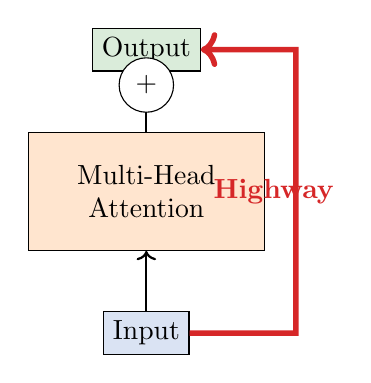
\begin{tikzpicture}[scale=0.9]
% Input
\node[draw, rectangle, fill=mlblue!20] (input) at (0,0) {Input};

% Attention block
\node[draw, rectangle, fill=mlorange!20, minimum width=3cm, minimum height=1.5cm, align=center] (attention) at (0,2) {Multi-Head\\Attention};

% Output
\node[draw, rectangle, fill=mlgreen!20] (output) at (0,4) {Output};

% Main path through attention
\draw[->, thick] (input) -- (attention);
\draw[->, thick] (attention) -- (output);

% Residual connection (highway)
\draw[->, thick, mlred, line width=2pt] (input.east) -- ++(1.5,0) -- ++(0,4) -- (output.east);
\node at (1.8,2) [mlred] {\textbf{Highway}};

% Addition symbol
\node at (0,3.5) [circle, draw, fill=white] {+};
\end{tikzpicture}
\end{center}

\vspace{3mm}
\begin{tcolorbox}[colback=mlblue!10,colframe=mlblue!75!black]
\textbf{Formula:} Output = Attention(Input) + Input
\end{tcolorbox}
\end{columns}

\vspace{3mm}
\begin{columns}[T]
\column{0.48\textwidth}
\begin{center}
\colorbox{yellow!20}{\parbox{0.9\columnwidth}{\centering
\textbf{Layer Normalization:}\\
Keeps signals in good range\\
(like adjusting volume)
}}
\end{center}

\column{0.48\textwidth}
\begin{center}
\colorbox{green!20}{\parbox{0.9\columnwidth}{\centering
\textbf{Why it works:}\\
If attention fails, original\\
information still flows through!
}}
\end{center}
\end{columns}
\end{frame}

% Slide 20: Complete Transformer Block
\begin{frame}{Everything Together: The Transformer}
\begin{center}
\includegraphics[width=0.75\textwidth]{../figures/3d_transformer_architecture.pdf}
\end{center}

\vspace{2mm}
\textbf{The Complete Pipeline:} All happens in parallel!
\begin{enumerate}
\item Words $\rightarrow$ Embeddings (positions in space)
\item Add positional encoding (wave patterns)
\item Multi-head attention (4 parallel perspectives)
\item Concatenate all heads
\item Feed-forward network
\item Output predictions
\end{enumerate}
\end{frame}

% Slide 20: Experimental Validation
\begin{frame}{Proof It Works: Real Results}
\begin{columns}[T]
\column{0.48\textwidth}
\textbf{Performance Comparison:}
\begin{center}
\begin{tabular}{|l|r|r|r|}
\hline
\textbf{Length} & \textbf{RNN} & \textbf{Transformer} & \textbf{Gain} \\
\hline
5 words & 95\% & 96\% & +1\% \\
20 words & 67\% & 89\% & +33\% \\
50 words & 31\% & 84\% & +171\% \\
100 words & 12\% & 81\% & +575\% \\
\hline
\end{tabular}
\end{center}

\vspace{3mm}
\textbf{Pattern:} Massive gains on long text!

\column{0.48\textwidth}
\textbf{Why the improvement:}
\begin{itemize}
\item No information bottleneck
\item Direct access to all words
\item Parallel computation
\item Multiple perspectives
\end{itemize}

\vspace{3mm}
\begin{tcolorbox}[colback=green!10!white]
\textbf{Validation:} The hypothesis works!
\end{tcolorbox}
\end{columns}
\end{frame}

% ===========================================
% PART 4: SYNTHESIS (5 slides)
% ===========================================

% Slide 21: Why Transformers Changed Everything
\begin{frame}{The Revolution: 2017-2024}
\begin{columns}[T]
\column{0.48\textwidth}
\textbf{Timeline of Innovation:}
\begin{itemize}
\item 2017: Original Transformer paper
\item 2018: BERT (understanding text)
\item 2019: GPT-2 (generating text)
\item 2020: GPT-3 (175B parameters)
\item 2022: ChatGPT (conversation)
\item 2023: GPT-4 (multimodal)
\item 2024: Claude, Gemini, Llama 3
\end{itemize}

\column{0.48\textwidth}
\textbf{Why it exploded:}
\begin{itemize}
\item Training 100x faster
\item Scales to billions of parameters
\item Works on any sequence data
\item Same architecture everywhere
\end{itemize}

\vspace{3mm}
\begin{tcolorbox}[colback=yellow!10!white]
One architecture conquered all of AI!
\end{tcolorbox}
\end{columns}
\end{frame}

% Slide 22: Core Insights
\begin{frame}{The Three Core Principles}
\vspace{3mm}
\begin{columns}[T]
\column{0.33\textwidth}
\begin{center}
\begin{tcolorbox}[colback=mlblue!10,colframe=mlblue!75!black,title={\centering\textbf{1. PARALLEL}}]
\textbf{Everything at Once}

\vspace{3mm}
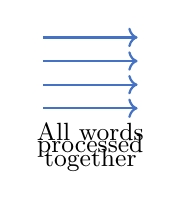
\begin{tikzpicture}[scale=0.6]
% Parallel arrows
\foreach \y in {0,0.5,1,1.5} {
    \draw[->,thick,mlblue] (0,\y) -- (2,\y);
}
\node at (1,-0.5) {\small All words};
\node at (1,-0.8) {\small processed};
\node at (1,-1.1) {\small together};
\end{tikzpicture}

\vspace{3mm}
\textbf{Result:}
\begin{itemize}
\item 100x faster
\item No bottlenecks
\item GPU efficient
\end{itemize}
\end{tcolorbox}
\end{center}

\column{0.33\textwidth}
\begin{center}
\begin{tcolorbox}[colback=mlgreen!10,colframe=mlgreen!75!black,title={\centering\textbf{2. ATTENTION}}]
\textbf{Focus on Relevant}

\vspace{3mm}
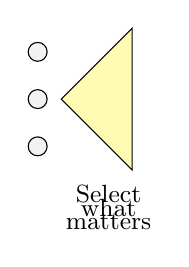
\begin{tikzpicture}[scale=0.6]
% Spotlight effect
\draw[fill=yellow!30] (0,0) -- (1.5,1.5) -- (1.5,-1.5) -- cycle;
\draw[fill=gray!10] (-0.5,1) circle (0.2);
\draw[fill=gray!10] (-0.5,0) circle (0.2);
\draw[fill=gray!10] (-0.5,-1) circle (0.2);
\node at (1,-2) {\small Select};
\node at (1,-2.3) {\small what};
\node at (1,-2.6) {\small matters};
\end{tikzpicture}

\vspace{3mm}
\textbf{Result:}
\begin{itemize}
\item Quality output
\item Noise filtering
\item Long-range deps
\end{itemize}
\end{tcolorbox}
\end{center}

\column{0.33\textwidth}
\begin{center}
\begin{tcolorbox}[colback=mlred!10,colframe=mlred!75!black,title={\centering\textbf{3. MULTI-HEAD}}]
\textbf{Multiple Perspectives}

\vspace{3mm}

\begin{tikzpicture}[scale=0.6]
% Four different views
\draw[thick,mlred] (0,1) -- (1,0);
\draw[thick,mlblue] (0,0.5) -- (1,0);
\draw[thick,mlgreen] (0,0) -- (1,0);
\draw[thick,mlorange] (0,-0.5) -- (1,0);
\node at (1,-1.5) {\small 4+ views};
\node at (1,-1.8) {\small combined};
\end{tikzpicture}

\vspace{3mm}
\textbf{Result:}
\begin{itemize}
\item Robust understanding
\item Different aspects
\item No blind spots
\end{itemize}
\end{tcolorbox}
\end{center}
\end{columns}

\vspace{5mm}
\begin{center}
\colorbox{yellow!20}{\parbox{0.8\textwidth}{\centering
\textbf{The Magic Formula:} Parallel Processing + Selective Attention + Multiple Perspectives = Transformers
}}
\end{center}
\end{frame}

% Slide 23: Real World Applications
\begin{frame}{Where You Use Transformers Every Day}
\begin{columns}[T]
\column{0.48\textwidth}
\textbf{Text:}
\begin{itemize}
\item ChatGPT conversations
\item Google search
\item Gmail autocomplete
\item DeepL translation
\end{itemize}

\vspace{3mm}
\textbf{Code:}
\begin{itemize}
\item GitHub Copilot
\item Cursor
\item Replit AI
\end{itemize}

\column{0.48\textwidth}
\textbf{Multimodal:}
\begin{itemize}
\item DALL-E (text to image)
\item Whisper (speech to text)
\item GPT-4V (vision)
\item Sora (text to video)
\end{itemize}

\vspace{3mm}
\textbf{Science:}
\begin{itemize}
\item AlphaFold (protein folding)
\item Weather prediction
\item Drug discovery
\end{itemize}
\end{columns}

\vspace{3mm}
\begin{center}
\colorbox{mlorange!20}{\textbf{All using the same transformer architecture!}}
\end{center}
\end{frame}

% Slide 24: Your Understanding Now
\begin{frame}{Check Your Understanding}
\begin{columns}[T]
\column{0.48\textwidth}
\textbf{You now understand:}
\begin{itemize}
\item[$\checkmark$] Words live in high-dimensional space
\item[$\checkmark$] Every word connects to every other
\item[$\checkmark$] Attention selects what's relevant
\item[$\checkmark$] Multiple heads = multiple perspectives
\item[$\checkmark$] Parallel processing enables scale
\item[$\checkmark$] Position encoding preserves order
\item[$\checkmark$] Same architecture powers ChatGPT
\end{itemize}

\column{0.48\textwidth}
\textbf{Quick Quiz:}

\vspace{3mm}
1. Why are transformers fast? \\
\colorbox{green!20}{Parallel processing}

\vspace{3mm}
2. What does attention do? \\
\colorbox{green!20}{Selects relevant information}

\vspace{3mm}
3. Why multiple heads? \\
\colorbox{green!20}{Different perspectives}
\end{columns}

\vspace{5mm}
\begin{center}
\colorbox{mlpurple!20}{\parbox{0.8\textwidth}{
\centering
\textbf{Congratulations!} You understand the technology behind ChatGPT! \\
From zero knowledge to transformer expert in 25 slides!
}}
\end{center}
\end{frame}

% Slide 25: Next Steps
\begin{frame}{Your Journey Continues}
\begin{columns}[T]
\column{0.48\textwidth}
\textbf{This Week's Lab:}
\begin{itemize}
\item Build attention mechanism
\item Implement multi-head attention
\item See the magic happen
\end{itemize}

\vspace{5mm}
\textbf{Next Week: Pre-training}
\begin{itemize}
\item How to train on internet scale
\item Why size matters
\item The emergence phenomenon
\end{itemize}

\column{0.48\textwidth}
\textbf{Key Takeaway:}

\vspace{3mm}
\begin{center}
\colorbox{mlblue!20}{\parbox{0.9\columnwidth}{
\centering
\textbf{Transformers =} \\
\vspace{2mm}
Parallel Attention \\
on All Words \\
with Multiple Perspectives
}}
\end{center}
\end{columns}

\vspace{5mm}
\begin{center}
{\Large \textbf{Questions?}}
\end{center}
\end{frame}

\end{document}